\section{Polyhedron Representation}\label{sec:preliminaries_poly}
% Conic
\begin{definition}
Given $k$ points $\vec{x}_1, \dots, \vec{x}_k \in \mathbb{R}^n$, any $\vec{x} = \sum_{i=1}^{k} \alpha_i \vec{x}_i$ is a \textbf{conic combination} of the $\vec{x}_i$, iff $\forall i \in \{1, \dots, k\}. \alpha_i \geq 0$.
\end{definition}

% Convexity
\begin{definition}\label{def:convex}
Given $k$ points $\vec{x}_1, \dots, \vec{x}_k \in \mathbb{R}^n$, any $\vec{x} = \sum_{i=1}^{k} \alpha_i \vec{x}_i$ is a \textbf{convex combination} of the $\vec{x}_i$, iff $\sum_{i=1}^{k} \alpha_i = 1 \land \forall i \in \{1, \dots, k\}. \alpha_i \geq 0$.

The set of all convex combinations of $\vec{x}_1, \dots, \vec{x}_k$ is therefore defined as:

\begin{equation*}
\conv(\vec{x}_1, \dots, \vec{x}_k) \coloneqq \left\{\sum_{i=1}^{k} \alpha_i \vec{x}_i \mid \sum_{i=1}^{k} \alpha_i = 1 \land \forall i \in \{1, \dots, k\}. \alpha_i \geq 0 \right\}
\end{equation*}
\end{definition}

\begin{corollary}\label{cor:intersection_convex}
The intersection of two convex sets is convex.
\end{corollary}

% Extreme Points
\begin{definition}
Let $\polyhedron{P}$ be a convex set. A point $\vec{p} \in \polyhedron{P}$ is an \textbf{extreme point} of $\polyhedron{P}$ if there is no non-trivial convex combination of any two points in $\polyhedron{P}$ expressing $\vec{p}$, i.e.:

\begin{equation*}
\forall \vec{x}_1, \vec{x}_2 \in \polyhedron{P}. \forall \alpha \in \mathbb{R}_+ \setminus \{0\}. \vec{x}_1 \neq \vec{x}_2 \implies \vec{p} \neq \alpha \vec{x}_1 + (1 - \alpha) \vec{x}_2
\end{equation*}
\end{definition}

% Rays
\begin{definition}\label{def:rays}
Let $\polyhedron{P}$ be a convex set. A vector $\vec{r} \in \mathbb{R}_0^n \setminus \{0\}$ is a \textbf{ray} of $\polyhedron{P}$ iff $\forall \vec{x} \in \polyhedron{P}. \forall \beta \in \mathbb{R}_+. \vec{x} + \beta \vec{r} \in \polyhedron{P}$.

The cone of rays $\vec{r}_1, \dots, \vec{r}_k \in \mathbb{R}_+^n$ is denoted as:

\begin{equation*}
\raycone(\vec{r}_1, \dots, \vec{r}_k) \coloneqq \left\{ \sum_{i=1}^{k} \alpha_i \vec{r}_i \mid \forall i \in \{1, \dots, k\}. \alpha_i \geq 0 \right\}
\end{equation*}
\end{definition}

\begin{definition}
A ray $\vec{r}$ of $\polyhedron{P}$ is an \textbf{extreme ray} of $\polyhedron{P}$ if there is no non-trivial conic combination of any two rays in $\polyhedron{P}$ expressing $\vec{r}$, i.e.:

\begin{equation*}
\forall \vec{r}_1, \vec{r}_2 \in \polyhedron{P}. \forall \alpha_1, \alpha_2, \beta \in \mathbb{R}_+ \setminus \{0\}. \vec{r}_1 \neq \beta \vec{r}_2 \implies \vec{r} \neq \alpha_1 \vec{r}_1 + \alpha_2 \vec{r}_2
\end{equation*}
\end{definition}

% Hyperplane
\begin{definition}
A \textbf{hyperplane} $\polyhedron{H} \subset \mathbb{R}^n$ of a $n$-dimensional space is a subspace of dimension $n-1$, and can therefore be described using a vector $\vec{f} \in \mathbb{R}^n$ and a scalar $f \in \mathbb{R}$ as $\polyhedron{H} = \{\vec{x} \mid \vec{f}\transpose \vec{x} = f\}$.
\end{definition}

\begin{corollary}
Any hyperplane is a convex set.
\end{corollary}

\begin{proof}
Let $\polyhedron{H} = \{\vec{x} \mid \vec{f}\transpose \vec{x} = f\}$ be a hyperplane. Let $k \in \mathbb{N}$, $\vec{x}_1, \dots, \vec{x}_k \in \polyhedron{H}$. For any $\alpha_1, \dots, \alpha_k \in \mathbb{R}_+$ with $\sum_{i=1}^{k} \alpha_i = 1$:

\begin{align*}
\vec{f}\transpose \left( \sum_{i=1}^{k} \alpha_i \vec{x}_i \right)
&= \sum_{i=1}^{k} \alpha_i \vec{f}\transpose \vec{x}_i \\
&= \sum_{i=1}^{k} \alpha_i \cdot f \\
&= f \cdot \sum_{i=1}^{k} \alpha_i \\
&= f
\end{align*}

Therefore, the convex combination $\sum_{i=1}^{k} \alpha_i \vec{x}_i$ is in the hyperplane $\polyhedron{H}$.
\end{proof}

% Halfspace
\begin{definition}
A \textbf{halfspace} is the set either above or below a hyperplane. A halfspace is open if the points on the hyperplane are excluded; otherwise, it is closed.
\end{definition}

\begin{corollary}\label{cor:halfspace_convex}
Any halfspace is a convex set.
\end{corollary}

\begin{proof}
Let $\polyhedron{H}^+ = \{\vec{x} \mid \vec{f}\transpose \vec{x} > f\}$ be an open halfspace (analogous for $\polyhedron{H}^- = \{\vec{x} \mid \vec{f}\transpose \vec{x} < f\}$, and for the closed halfspaces). Let $k \in \mathbb{N}$, $\vec{x_1}, \dots, \vec{x_k} \in \polyhedron{H}^+$. For any $\alpha_1, \dots, \alpha_k \in \mathbb{R}_+$ with $\sum_{i=1}^{k} \alpha_i = 1$:

\begin{align*}
\vec{f}\transpose \left( \sum_{i=1}^{k} \alpha_i \vec{x}_i \right)
&= \sum_{i=1}^{k} \alpha_i \vec{f}\transpose \vec{x}_i \\
&> \sum_{i=1}^{k} \alpha_i \cdot f \\
&= f \cdot \sum_{i=1}^{k} \alpha_i \\
&= f
\end{align*}

Therefore, the convex combination $\sum_{i=1}^{k} \alpha_i \vec{x}_i$ is in the halfspace $\polyhedron{H}^+$.
\end{proof}

% Polyhedron
\begin{definition}
A \textbf{polyhedron} $\polyhedron{P} \subseteq \mathbb{R}^n$ is defined by the intersection of a set of closed halfspaces, i.e., $\polyhedron{P} \coloneqq \{\vec{x} \in \mathbb{R}^n \mid \mat{A} \vec{x} \geq \vec{b}\}$, with $\mat{A} \in \mathbb{R}^{m \times n}, \vec{b} \in \mathbb{R}^m$.
\end{definition}

\begin{corollary}
A polyhedron is a convex set.
\end{corollary}

\begin{proof}
Follows from Corollaries \ref{cor:intersection_convex} and \ref{cor:halfspace_convex}.
\end{proof}

% Monkowski-Weyl
\begin{definition}
The \textbf{Minkowski sum} of two sets $P, Q$ is defined by:
\begin{equation*}
P \oplus Q \coloneqq \left\{\vec{p} + \vec{q} \mid \vec{p} \in P \land \vec{q} \in Q \right\}
\end{equation*}
\end{definition}

\begin{theorem}[Minkowski-Weyl \cite{chappell2019minkowski,thebook}]\label{th:minkowski-weyl}
For $\polyhedron{P} \subseteq \mathbb{R}^n$ the following statements are equivalent:

\begin{enumerate}
\item $\polyhedron{P}$ is a polyhedron, i.e., there exists some finite matrix $\mat{A} \in \mathbb{R}^{m \times n}$ and some vector $\vec{b} \in \mathbb{R}^m$ such that $P = \{\vec{x} \in \mathbb{R}^n \mid \mat{A} \vec{x} \leq \vec{b}\}$
\item There exist fine vectors $\vec{v}_1, \dots, \vec{v}_s \in \mathbb{R}^n$ and finite vectors $\vec{r}_1, \dots, \vec{r}_t \in \mathbb{R}_+^n$, such that $P = \conv(\vec{v}_1, \dots, \vec{v}_s) \oplus \raycone(\vec{r}_1, \dots, \vec{r}_t)$
\end{enumerate}
\end{theorem}

In simple terms, the Minkowski-Weyl theorem states that any polyhedron can always be defined in two ways: either by its faces, i.e., closed halfspaces, or by its vertices and rays. Most polyhedra can be represented in this way using only their extreme points and extreme rays. Figure \ref{fig:minkowski-weyl} illustrates this theorem on two exemplary polyhedra.

\begin{figure}
\centering
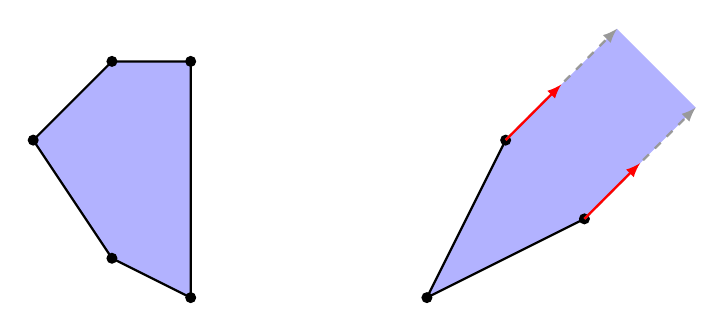
\begin{tikzpicture}
% Define the extreme points
\coordinate (A) at (-4,0.5);
\coordinate (B) at (-5,2);
\coordinate (C) at (-4,3);
\coordinate (D) at (-3,3);
\coordinate (E) at (-3,0);

% Draw the filled region
\fill[fill=blue!30] (A) -- (B) -- (C) -- (D) -- (E) -- cycle;

% Draw the extreme points
\foreach \point in {A, B, C, D, E}
  \fill[black] (\point) circle (2pt);

% Draw the edges of the polyhedron
\draw[thick] (A) -- (B) -- (C) -- (D) -- (E) -- cycle;

%%%%%%%%%%

% Define the extreme points
\coordinate (A) at (1,2);
\coordinate (B) at (0,0);
\coordinate (C) at (2,1);

% Define the ends of the rays
\path (A) -- +(45:2cm) coordinate (A-ray);
\path (C) -- +(45:2cm) coordinate (C-ray);
\path (A) -- +(45:1cm) coordinate (A-ray-short);
\path (C) -- +(45:1cm) coordinate (C-ray-short);

% Draw the filled region
\fill[fill=blue!30] (A) -- (B) -- (C) -- (C-ray) -- (A-ray) -- cycle;

% Draw the extreme points
\foreach \point in {A, B, C}
  \fill[black] (\point) circle (2pt);

% Draw the edges of the polyhedron
\draw[thick] (A) -- (B) -- (C);

% Draw rays from points (1,2) and (2,1)
\draw[dashed, thick, gray!80, -latex] (A) -- (A-ray); % Ray at 45 degrees from point (1,2)
\draw[dashed, thick, gray!80, -latex] (C) -- (C-ray); % Ray at 45 degrees from point (2,1)
\draw[thick, red, -latex] (A) -- (A-ray-short); % Ray at 45 degrees from point (1,2)
\draw[thick, red, -latex] (C) -- (C-ray-short); % Ray at 45 degrees from point (2,1)
\end{tikzpicture}
\caption{Illustration of the Minkowski-Weyl theorem. The left figure shows a fully bounded polyhedron represented by its extreme points. Unbounded polyhedra, such as the one on the right, require extreme rays, shown in red, for a complete description.}
\label{fig:minkowski-weyl}
\end{figure}

The following theorem builds upon the Minkowski-Weyl theorem to describe a polyhedron, which is represented by its extreme points $\{\vec{x}_p\}_{p \in P}$ and extreme rays $\{\vec{x}_r\}_{r \in R}$, using hyperplanes. Here, the sets $P, R$ are used to index the extreme points and extreme rays, respectively.

\begin{theorem}[Nemhauser-Wolsey \cite{wolsey2014integer,thebook}]\label{th:nemhauser-wolsey}
Consider the polyhedron $\polyhedron{P} = \{\vec{x} \in \mathbb{R}^n \mid \mat{Q} \vec{x} \geq \vec{b}\}$ with full row rank matrix $\mat{Q} \in \mathbb{R}^{m \times n}$, i.e., $\rank(\mat{Q}) = m \leq n \land \polyhedron{P} \neq \emptyset$.

An equivalent description of $\polyhedron{P}$ using its extreme points $\{\vec{x}_p\}_{p \in P}$ and extreme rays $\{\vec{x}_r\}_{r \in R}$ is:

\begin{equation}
\polyhedron{P} = \left\{ \vec{x} \in \mathbb{R}^n \middle\vert
\begin{aligned}
\sum_{p \in P} \vec{x}_p \lambda_p &+ &\sum_{r \in R} \vec{x}_r \lambda_r &= \vec{x} &\\
\sum_{p \in P} \lambda_p & & &= 1 &\\
\lambda_p & & &\geq 0 &\forall p \in P\\
& &\lambda_r &\geq 0 &\forall r \in R
\end{aligned}
\right\}
\end{equation}
\end{theorem}

The conditions of the Minkowski-Weyl theorem are clearly encoded in the Nemhauser-Wolsey theorem: the second and third lines ensure that the convex set of the extreme points is considered in the first line (Definition \ref{def:convex}), the last pertains to the cone of extreme rays (Definition \ref{def:rays}), and the first line represents the Minkowski sum of the convex hull of extreme rays and the cone of extreme rays.

By requiring $\vec{x} \in \mathbb{Z}^n$ in Theorem \ref{th:nemhauser-wolsey}, we can also describe the integral polyhedra using possibly fractional extreme points and rays. Alternatively, the Nemhauser-Wolsey theorem has been adapted to describe integral polyhedra using only integral (interior) points and (integer-scaled) extreme rays, as shown in the following theorem.

\begin{theorem}[Nemhauser-Wolsey \cite{wolsey2014integer,thebook}]\label{th:nemhauser-wolsey-integer}
Consider the polyhedron $\polyhedron{P} = \{\vec{x} \in \mathbb{R}^n \mid \mat{Q} \vec{x} \geq \vec{b}\}$ with full row rank matrix $\mat{Q} \in \mathbb{R}^{m \times n}$, i.e., $\rank(\mat{Q}) = m \leq n \land \polyhedron{P} \neq \emptyset$. Have $\polyhedron{Q} \coloneqq \polyhedron{P} \cap \mathbb{Z}^n \neq \emptyset$ be the integer hull of $\polyhedron{P}$.

An equivalent description of $\polyhedron{Q}$ using a finite subset $\{\vec{x}_p\}_{p \in \ddot{P}}$ of its integer points and its (integer-scaled) extreme rays $\{\vec{x}_r\}_{r \in R}$ is:

\begin{equation}
\polyhedron{Q} = \left\{ \vec{x} \in \mathbb{Z}^n \middle\vert
\begin{aligned}
\sum_{p \in \ddot{P}} \vec{x}_p \lambda_p &+ &\sum_{r \in R} \vec{x}_r \lambda_r &= \vec{x} &\\
\sum_{p \in \ddot{P}} \lambda_p & & &= 1 &\\
\lambda_p & & &\in \{0, 1\} &\forall p \in \ddot{P}\\
& &\lambda_r &\in \mathbb{Z}_+ &\forall r \in R
\end{aligned}
\right\}
\end{equation}
\end{theorem}

\begin{note}\label{note:nemhauser-wolsey}
A notable difference between the Nemhauser-Wolsey theorem for real polyhedra and integral polyhedra is that for the former it suffices to use extreme points and extreme rays, while for the latter, interior points of $\polyhedron{Q}$ might be required to describe the integer hull $\polyhedron{Q}$.
\end{note}
